\section{Introduction}
Unmanned Aerial Vehicles (UAV) are gaining popularity in private as well as commercial sector. One often-mentioned use-case is the parcel delivery. In the near future, UAV might be used to deliver parcels to your doorstep. The logistics industry hopes for positive impacts on their costs and competitiveness. The deployment of a delivery concept is quite complex. To allow for early evaluation and reduce the number of required flight-testing, a simulation engine is required. This is why SIMULATIONNAME has been developed. It supports multiple depots and UAV as well as  simple change of path-planning algorithm. UAVs move in a 3D environment  The engine does not simulate the behaviour of the UAV in the aerial space itself but allows for evaluation of spatial distribution of depots or the suitability of a path-planning algorithm. It was developed considering the use of swarm algorithms in the delivery use-case and allow for inter-drone communication and autonomous organisation avoiding a central ground control.

\section{Related Work}
The literature on simulation engines for a UAV parcel delivery scenario is still relatively scarce. In general the researchers concentrate more on specific components or fight behavior rather than the whole delivery use case. Eric Johnson and Sebastien Fointaine developed a simulation engine for the behavior of specific hardware components of a UAV \cite{johnson.2001}. Their research focuses mainly on low-cost UAVs with limited capacities. The simulation provides high benefit for minimal effort and enables simulations with reasonable costs, taking into account the limited resources of the UAVs without accessing the UAVs actual hardware. Lu and Geng (2011) simulated the flight dynamic behavior of a UAV using Matlab/Simulink focusing on the control law of UAVs \cite{lu.2011}. They propose a Hardware-In-a-Loop (HIL) simulation based on a mathematical UAV model, that includes the characteristics of the UAV. The simulation shows very low deviations between the system and real flights and is therefore suitable to test and validate the control law designs of a UAV. \\
MultiUAV \cite{rasmussen.2003}, a very general simulation engine has been developed to simulate cooperative algorithms for finding targets. The software includes not only vehicle dynamics but also flight dynamics, that is based on cooperative control algorithms. The cooperative control of UAVs requires an implementation of a inter-vehicle communication which is also addressed in our research. Furthermore, an agent-based simulation engine implementing a surveillance scenario was introduced in 2005\cite{jang.2005}. The main goal of this research was to develop efficient coordination methods for large-scale multi-agent systems. The simulation shares some similar concepts with the simulation proposed in our paper. For example, in their scenario the UAVs try to find targets without prior knowledge of the targets’ locations. The UAVs are implemented as autonomous agents that interact with each other via messages. Moreover, the notion of obstacles and bases is being used. The described sensor concept is also similar to the one used in this paper.

\section{Scenario}
NO CENTRAL ENTITY, optimizes
\\
Before embarking the software model, the delivery scenario shall be described.  Every UAV has a depot, in the engine called basestation, from which it receives items to be delivered. An item's destination is within the range of a Basestation which means that every Basestation has a limited range in the area. UAVs are assigned to one specific Basestation and only deliver items of it. After receiving an item, the UAV will begin flying to the specific destination. It scans the area and stores information on all fields it has seen en-route. If a UAV meets another one, they will exchange information on the already-explored parts of the area.\\
If a field on the route contains an obstacle, it will deviate from its route and try to find one around the obstacle. Obstacles can have different heights, thus UAV als\\
After delivering the item, it will fly back to the basestation to receive a new item. If the battery reaches a certain threshold, the UAV will fly to the nearest basestation (not neccessarily its home base) and recharge its battery. 
 UAVs are moving in a 3D environment which means that obstacles can have different heights.

\section{Description of the model}
The simulation has been written in Python, using the MESA framework for agent-based modelling. Figure \ref{fig:architecture} represents the software architecture. There are three major components: the simulation model itself, implementing the simulation environment and logic, an analytics interface for evaluating a simulation's performance and the GUI realized using a web server and allowing for easy access with a standard web-browser. The UAV as part of the simulation model, shall be described in particular in section \ref{sec:UAV}.\\
The simulation's aim is to support comparing of different decentralized path-planning algorithms by making them easily exchangeable. Predefined KPI's and an output method are used to support analyzing the performance of one's implementation. Section \ref{sec:KPI} discusses the way KPI's are defined.\\
\begin{figure}[htbp]\label{fig:architecture}
	\centering
	\includegraphics[scale=0.2]{images/architecture.png} 
	\caption{Architecture of simulation model}
\end{figure}
Figure \ref{fig:architecture} shows the architecture of the simulation model. In general, the model contains of a UI component including configurationa and GUI, the model containing the UAV, the world model and the programming logic and the data analysis component which writes out the simulation results to allow for further evaluation. 


\subsection{MESA}
MESA \cite{masad.2015} is an open source agent-based modeling framework (ABM) developed specifically for the Python programming language.  Agents are objects that have rules and states that act accordingly on every step of the simulation \cite{axtell.2000}. ABM allows to capture the path of the simulation along with the solution and allows for analysing the dynamic history \cite{axtell.2000}. ABM also allows to dynamically pause and resume the simulation at any given step and analyse the current results.\\
MESA comes with implementations of important components, such as a grid for implementing a simple 2D environment, a web-browser-based UI, a data analysis tool and an agent scheduler. It allows for easy extension or modifications to develop specific simulation engines. \\
Our simulation uses all core components of MESA, such as the MultiGrid, the DataCollector, the scheduler (RandomActivation), agents and the server component \cite{masad.2015}:
\begin{itemize}
	\item The MultiGrid is a 2D grid with fields that allow for more than one agent on one field. This is particularly important for our simulation as agents of different height are all stored in the same grid in the model.
	\item The DataCollector is used for collecting relevant quantitative data to support the evaluation of an algorithm.
	\item The scheduler activates the agents. An agent will only do an action if the scheduler activates it. We use the RandomActivation which means that in every step the agents are activated in a random order.
	\item The server renders the graphical user interfaces and renders changes on the model. It also allows for pausing and resuming the simulation or progress step-wise. 
\end{itemize} 
\begin{itemize}
	\item Which components did we remove or modify and why?
	\item In order to optimize rendering performance, some modifications to the user interface components of MESA have been made. For example, an explicit "Obstacle" class is not required anymore as the MultiGrid was modified to not store whole objects with attributes anymore but using numerical codes to identify obstacles or depots. Storing the actual agents in the grid was not required anymore as the model keeps a collection of depots (in the simulation called "BaseStations") in the scheduler and thus did not require for the grid to store those information anymore. The GUI itself parses an image file and does not require information on the actual objects inside the simulation model.
	\item Reprogramming of rendering engine. How and why?
\end{itemize}



\subsection{User Interface: Configuration and GUI}
The user interface consists of two parts: The file \textit{config.ini} to change the simulation scenario and a web server responsible for rendering the GUI and delivering it through a web browser.\\
The configuration file is being parsed at the startup of the simulation engine and contains all the required settings for the simulation to work properly. It contains crucial information that have a high impact on an algorithm's performance and makes it easy to set up different scenarios, e.g. one might consider testing the results using different number of UAVs per depot or more or less depots itself.
Furthermore the impact of different battery capacity (in steps) can easily be simulated. A higher sensor range can be beneficial for an algorithm's performance but should be chosen realistically according to the model.\\
As mentioned earlier, the GUI is implemented using a web server. For the GUI to properly function, two image files are required. One contains the map as the user is supposed to see it. The other one stores information on obstacles and their respective heights using color codes. White means that there is no obstacle and other colors represent different altitude levels. An obstacle is any static object (such as trees or buildings etc.) that obstructs the movement of the UAV. The file will be parsed on start-up and the information stored in the model.  Depots are placed on obstacles.\\
The GUI allows for starting, pausing and resetting the simulation and shows the movement of UAVs in the space. It is implemented in a 2D fashion although internally the model calculates with 3-dimensional coordinates. The image's color codes for obstacles are used to represent the different altitudes. For now, the simulation tool supports 5 different height levels but one can easily modify the parser and define more colors for more altitude levels.
To receive immediate information on UAV without waiting for the simulation to reach an amount of desired steps, one can click on a UAV, receive position and destination information as well as battery status. Figure \ref{fig:uav_detail} shows this view.



	\begin{figure}[htbp]\label{fig:uav_detail}
		\centering
		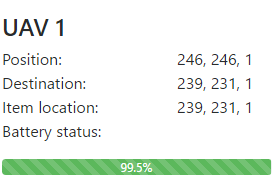
\includegraphics[scale=0.5]{images/uav_detail.png}
		\caption{Detailed view of UAV information}
	\end{figure}


\subsection{Agents}\label{sec:UAV}
The most important agent of a UAV simulation is the UAV itself. We developed a realistic simulation representing the required components and behavior and omitted not required components to cover the delivery scenario. The simulated UAV has the following components:
	\begin{itemize}
			\item Battery: The battery has a limited battery life that decreases on each step. When the battery reaches a certain threshold (configurable), the UAV will fly to the nearest depot to recharge.
					\item CargoBay: The cargoBay represents the UAV's storage unit which can contain exactly one item.
		\item FlightController: This component contains the path-finding/route-planning algoritm. It represents a navigation unit. Multiple algorithms could be implemented, compare section \ref{sec:algorithm} for an example. The algorithm uses the sensor to identify its neighboring fields at any step. Additionally it stores a perceived world which holds all fields that are already explored. 
		\item CommunicationModule: If the sensor found another UAV in the sensor's radius, this component will communicate with the other UAV and exchange grid information. Exchange of information on previously-unknown terrain helps when a UAV has to deliver an item to a new area of the map. This allows for precomputing optimal routes before exploring the actual area.
		\item Sensor: Scanning the grid for obstacles and other agents. This component is the interface to the model
	\end{itemize}

UAVs do not communicate with a central entity such as a control server organizing the flight traffic. They communicate with each other if they are in sensor range and only rely on their own sensor.
To optimize performance for the exchange of grids, the UAVs only store a dictionary containing their perceived world rather than a full matrix implemented in MESA's grid.
There is one dictionary for each height level, mapping coordinates to information whether there is an obstacle on that field or not.  
\\
The second agent in the simulation is the BaseStation. In the real world, this is the depot of a logistics company. It assigns orders to UAVs and hands items over to them. Depots are responsible for all items in a part of the map and for a subset of all drones. Also, they contain chargers for UAVs whose battery reached a low level. In the configuration, one can set how many depots are supposed to be on the map by specifying the number of fields the depot is responsible for (its delivery area). Depots are located as close to the center of their area as possible, but only on obstacles (on buildings). Items that are picked up from a depot can have different priorities in order to make the simulation more realistic. For example, items with high priority can be important and immediately required medical equipment or parcels for which a customer paid a higher fee to receive it faster.



\subsection{Analytics}\label{sec:KPI}
During a run, data and results are being generated. To allow for the evaluation of a path finding algorithm
For evaluating the delivery scenario, we identified the following KPI's:
\begin{itemize}
	\item Average walk length: Describes the average number of steps taken for an item to be delivered. 
	\item Average walk length divided by initial distance: This data point is a ratio calculated by dividing the average number of steps taken by the initial distance from base station to an item's destination. The initial distances are calculated as euclidean distances. Example: A value of 2 means that the average walk length is 2 times the initial distances.
	\item Standard deviation of average walk lengths: Represents the standard deviation of all walk lengths to get a better insight into the data additional to the average walk length.
	\item Items delivered per UAV: Items delivered divided by number of UAV's.
	\item Average lifetime of item: Calculation of the average lifetime of items by aggregating all item's lifetimes, divided by number of items. Lifetime is defined as the time from being available for delivery at the depot to the actual delivery at the item's destination.
\end{itemize}

The results are step-wise written out into a CSV file during the simulation and can for example be imported into a spreadsheet software or more sophisticated tools like R or any other application to run statistical analysis of the KPI's. Technically, this is realized by using MESA's DataCollector class. This allows for easy definition of values to be calculated every step and export them to a CSV file. The KPI's can easily be extended or modified in the source code.

\begin{figure}[htbp]
	\centering
	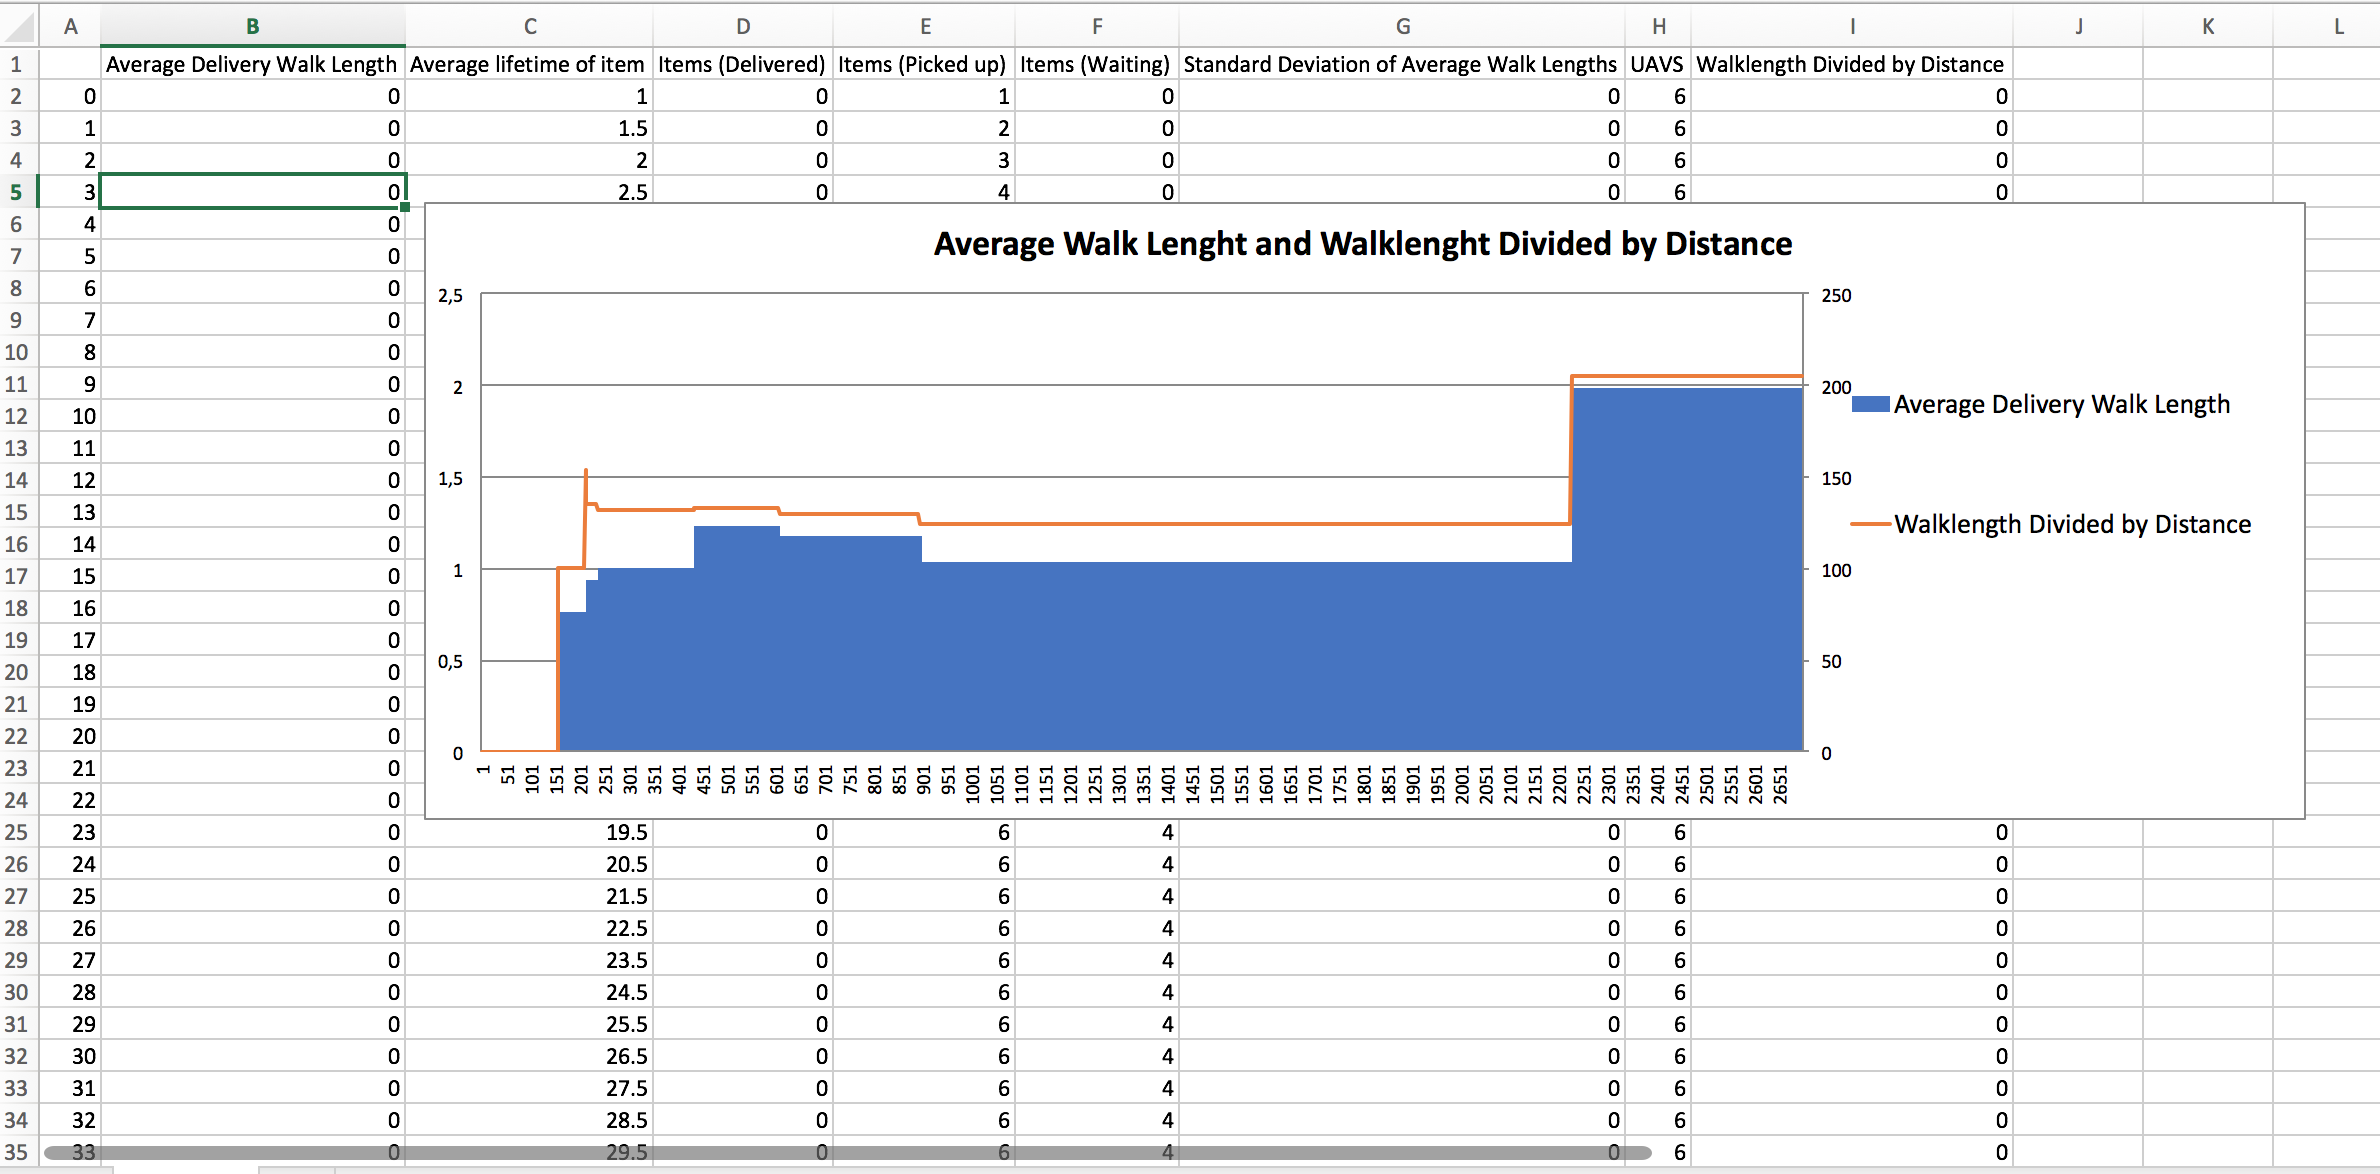
\includegraphics[scale=0.4]{images/walk}
	\caption{Example of analyzing KPI's in a spreadsheet software}
\end{figure}



\section{Implementation of a sample algorithm: A Star}\label{sec:algorithm}
To provide an example simulation, the A* algorithm has been used 
SOURCES!


\section{Evaluation}
The simulation engine presented in this paper allows for a simple evaluation of a path planning algorithm in a 3-dimensional space. Also it helps to implement traditional algorithms into a swarm optimization problem as UAVs exchange their grid whenever they come close enough to each other. A bottleneck is the calculation performance. On a mid-2015 Apple Macbook Pro with a i5 Dual core processor, the simulation of 5000 steps (run without GUI) still takes a very long time. This is due to the fact that the implementation of the MESA grid used in the model is not performance-optimized. Also, the exchange of the grid is a complex task. It was tried to optimize performance by using dictionaries for the UAV's perceived world rather than storing a complete matrix. The model's internal grid also has been modified to just store numerical values for obstacles (1+ altitude), baseStations/depots (-1) or 0 for no content.

\section{Conclusion}
This paper presented a new simulation engine specifically developed for the delivery use-case with autonomous UAV not being controlled by a central control server. Delivery of items will be relevant in the near future and a simulation engine is required to test for different scenarios, such as different numbers of depots or rural against urban regions. The engine supports multiple depots and UAVs, communication between UAV and different altitude levels for testing. It is based on the MESA modeling framework whereas many adjustments for performance have been implemented. The GUI allows for visual evaluation of the simulation's progress and the CSV output helps analyzing the final scenario results. The simulation of a battery helps to understand how far a destination should be from a depot and thus how many depots are required. \\
The engine does not support UAVs carrying more than one item nor changing the input file for the map. Currently it comes with an example map but in the future this should be exchangeable. An example algorithm was implemented



